\documentclass{article}

\usepackage{caption}
\usepackage{subcaption}
\usepackage{graphicx}
\usepackage{tikz}
\usepackage{tikzsymbols}
\usetikzlibrary{calc}
\usepackage{float}
\usepackage{pdflscape}
\usepackage{geometry}
\geometry{a4paper, landscape, margin=1cm}


\def\centerarc[#1](#2)(#3:#4:#5){\draw[#1] ($(#2)+({#5*cos(#3)},{#5*sin(#3)})$) arc (#3:#4:#5);}


\pagestyle{empty}
\begin{document}
	\centering
	\begin{figure}[H]
			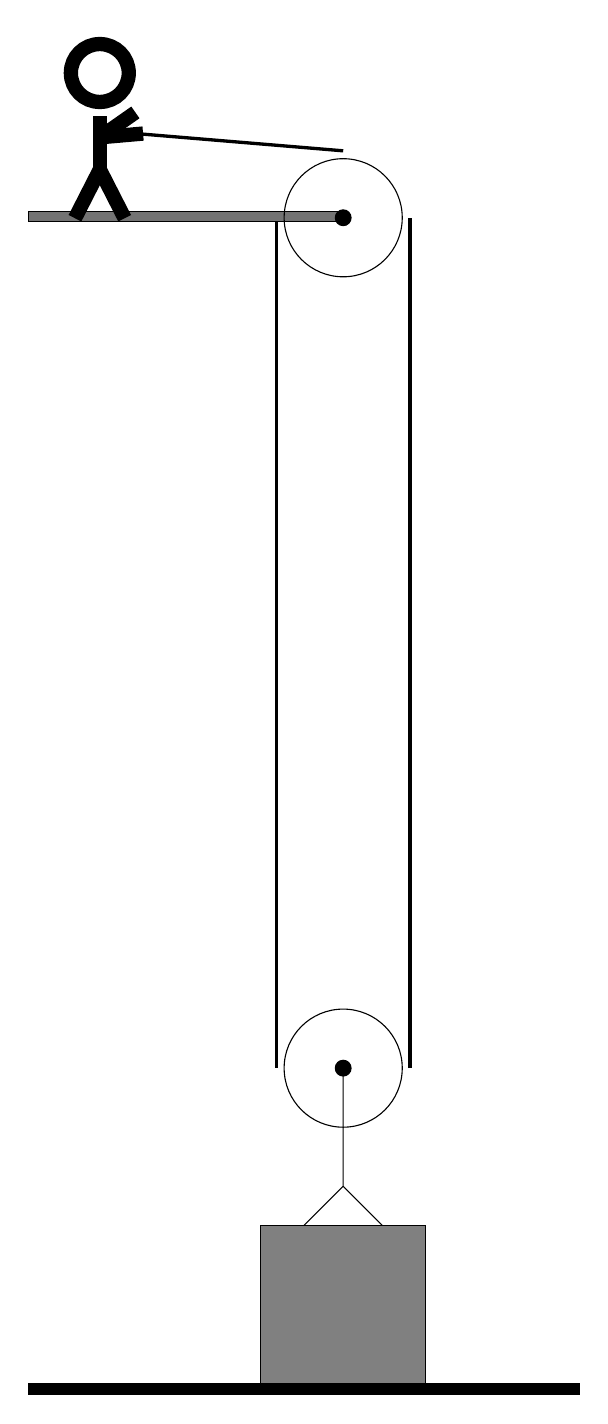
\begin{tikzpicture}
				%%%%% START %%%%%
				\def\a{11.75}
				\def\radlg{0.75}
				\def\radrp{0.85}
				\def\radsm{0.1}
				\def\yone{1}
				\def\xone{2}
				\def\ytwo{11.8}
				\def\xtwo{2}
				\def\dx{-1}
				\def\dy{12.9}
				\def\dw{1.75mm}
				
				\draw[fill=black!55] (-2,\a) rectangle (\xtwo,\a+0.125);
				
				\draw (\xone,\yone) circle (\radlg);
				\draw[fill=black] (\xone,\yone) circle (\radsm);
	
				\draw (\xtwo,\ytwo) circle (\radlg);
				\draw[fill=black] (\xtwo,\ytwo) circle (\radsm);
				
				\draw (\xone,\yone) -- (\xone,\yone-1.5) -- (\xone-0.5,\yone-2) -- (\xone+0.5,\yone-2) -- (\xone,\yone-1.5);
				\draw[fill=black!50] (\xone-1.05,\yone-2) rectangle (\xone+1.05,\yone-4);  
				
				\draw[very thick] (\xone-\radrp,\a) -- (\xone-\radrp,\yone); 
				\centerarc[very thick](\xone,\yone)(180:360:\radrp);
				\draw[very thick](\xone+\radrp,\yone) -- (\xtwo+\radrp,\ytwo);
				\centerarc[very thick](\xtwo,\ytwo)(0:90:\radrp);
				\draw[very thick](\xtwo,\ytwo+\radrp) -- (\dx,\dy);
					
				\node at (\dx,\dy) {\Strichmaxerl[10][-175][35]};
				
				\draw[fill=black] (-2,-3) rectangle (5,-3.15);
				%%%%% END %%%%%
			\end{tikzpicture}
	\end{figure}
	
\end{document}